\chapter{TODO: 1st lecture missing}

\begin{descr}
    TODO
\end{descr}

\section{TODO}\index{TODO}
\begin{definition}
    TODO
\end{definition}
\begin{definition}
    TODO
\end{definition}
\begin{definition}
    TODO
\end{definition}
\begin{lemma}
    TODO
\end{lemma}

\begin{definition}
    Let $G = (V,E)$ be a graph without loops. If there exists $V_{1}, V_{2} \leq V$ and $V_{1} \cup V_{2} = V$
    such that $V_{1} \cap V_{2} = \emptyset$ and every edge $e$ has one endpoint in $V{_1}$ and the other in $V_{2}$,
    then we call $G$ a \deftxt{bipartite}.
\end{definition}

\begin{example*}
    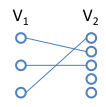
\includegraphics{diagrams/def14_example1.png}
\end{example*}

\begin{definition}
    A directed graph is a pair $G = (V,E)$ where $V$ is a set of nodes (vertices) and $E$ is a set of edges together 
    with a function $i: E -> V x V$. If $i(e) = (v_{1},v_{2})$ then $v_{1}$ is called start point, $v_{2}$ is called end point.
\end{definition}
Graphically: \\[3mm]
If $i(e) = (v_{1},v_{2})$ we draw 1. \\
If $i(e') = (v_{1},v_{2})$ then this indices a second edge (2.). \\
If $i(e_{1}) = i(e_{2})$ we call $e_{1},e_{2}$ parallel. \\
If $i(e) = (v,v)$ then $e$ is called a directed loop. \\
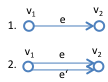
\includegraphics{diagrams/def15_directd_graph.png} \\
$g_{out}(v)$ is the number of edges that have starting point $v$. \\
$g_{in}(v)$ is the number of edges with endpoint $v$.

\begin{lemma}
    $\displaystyle\sum\limits_{v \in V} g_{in}(v) = \displaystyle\sum\limits_{v \in V} g_{out}(v)$
\end{lemma}

\begin{prooof}
    We start with a graph without edges. Then we insert one after the other edges in $E$. 
    Each edge contributes 1 to both sides of the equation.
\end{prooof}

\begin{definition}
    A directed path is a sequence of edges $e_{1},e_{2}...$ such that the end point of $e_{i}$ is the start point of
    $e_{1} +1, i > 1$([NW] +1 seems strange to me, correct?). \\[3mm]

    A directed path $e_{1}...e_{k}$ is called a (directed) \underline{cycle}, if the start point of $e_{1}$ and
    the end point of $e_{k}$ coincide. \\
    A simple (directed) path is a path where every node occurs at most once. \\
    A directed cycle is called simple if every node except for the start and end node occurs at most once.
\end{definition}

\begin{definition}
    A graph directed or undirected is called \underline{simple}, if it does not contain parallel edges.
\end{definition}

\begin{definition}
        A directed graph is called \underline{strongly connected} if for any pair of nodes $(u,v)$ 
        there is a directd path from $u$ to $v$.
\end{definition}

Let $G$ be a directed graph $G = (V,E)$. $x,y \in V x~y$ ([NW] does ~ mean are "connected"?)
if there is a directed path from x to y and vice versa. \\

The equivalence classes of this relation $~c VxV$ are called strongly connected components.
(Analogously: Define connected components for undirected graphs)

\begin{information}
    We should know how the following terms are defined: reflexivity, symetry, transitivity.
\end{information}


